%! suppress = TooLargeSection
\documentclass[12pt]{article}

\usepackage{url,amsmath,setspace,amssymb}
\usepackage{fancyvrb}
\usepackage{fvextra}
\usepackage{listings}
\usepackage{graphicx}
\usepackage{tcolorbox}
\usepackage{tikz}
\usepackage{xcolor}
\usepackage{caption}
\usepackage{color}
\usepackage{cite}
\usepackage{xassoccnt}
\usepackage{subcaption}
\usepackage{hyperref}

\NewTotalDocumentCounter{totalpages}
\DeclareAssociatedCounters{page}{totalpages}

\newcommand{\studentname}{Francesco Bombassei De Bona}
\newcommand{\studentnumber}{144665}

\setlength{\oddsidemargin}{.25in}
\setlength{\evensidemargin}{.25in}
\setlength{\textwidth}{6.25in}
\setlength{\topmargin}{-0.4in}
\setlength{\textheight}{8.5in}

\renewcommand{\thepage}{10-\arabic{page}}
\newcommand{\heading}[5]{
    \noindent
    \begin{center}
        \framebox[\textwidth]{
            \begin{minipage}{0.9\textwidth} \onehalfspacing
            {\textbf \unitname} \hfill #1

                {\centering \Large #4

            }\medskip
            {#2 \hfill #3}
            \end{minipage}
        }
    \end{center}
}

\newcommand{\unitname}{Automated Reasoning}
\newcommand{\handout}{\heading{A.A. 2021/2022}{\studentname}{\studentnumber}{Relazione di progetto}}

\begin{document}
    \handout{}

    \section{Outline}\label{sec:outline}
    In questa relazione analizzerò il problema proposto per lo svolgimento del progetto di Automated Reasoning, proporrò una soluzione al problema codificata in Minizinc e una soluzione codificata in ASP.
    Inoltre, analizzerò i risultati ottenuti con entrambe le soluzioni e le differenze tra i due approcci.

    \section{Struttura del progetto}\label{sec:struttura-del-progetto}
    La struttura del progetto è la seguente:
    \begin{itemize}
        \item \textbf{report}: contiene il report del progetto;
        \item \textbf{asp}: contiene il codice ASP;
        \item \textbf{minizinc}: contiene il codice MiniZinc;
        \item \textbf{python}: contiene il codice Python per la generazione di grafici e per la generazione delle visualizzazioni delle soluzioni;
        \item \textbf{results}: contiene i risultati dei benchmark salvati in formato \emph{json};
        \item \textbf{benchmark.c}: contiene il codice per lanciare i benchmark;
        \item \textbf{setup.c}: contiene il codice per generare le istanze casuali del problema.
    \end{itemize}

    In particolare le cartelle \emph{asp} e \emph{minizinc} contengono le seguenti sottocartelle:
    \begin{itemize}
        \item \textbf{data}: contiene le istanze del problema;
        \item \textbf{results}: contiene le visualizzazioni create con Python dei risultati dei benchmark.
    \end{itemize}

    \section{Problema}\label{sec:Problema}
    Sia data una griglia quadrata di lato \emph{n} e sia dato un certo numero di carte di cui si consideri il segno $\clubsuit$, $\heartsuit$, $\spadesuit$, $\diamondsuit$.
    Il numero di carte per ogni seme può essere diverso da quello standard (tredici per seme).
    Alcune celle sono già occupate, alcune celle sono bloccate/vietate (indicate con il simbolo $\square$), ogni cella libera può contenere al più una carta, e non vi possono essere più di tre carte adiacenti dello stesso seme.
    L'obiettivo è disporre le carte disponibili in modo da massimizzare il punteggio ottenuto dalle seguenti regole:
    \begin{itemize}
        \item due carte adiacenti dello stesso seme (orizzontali e/o verticali): 1 punto;
        \item tre carte adiacenti dello stesso seme (orizzontali e/o verticali): 3 punti;
        \item se si conta la terna non si contano le due coppie;
        \item quattro carte adiacenti disposte in verticale di quattro semi diversi: 4 punti;
        \item quattro carte adiacenti disposte in orizzontale di quattro semi diversi: 6 punti.
    \end{itemize}

    \begin{figure}[h]
        \centering
        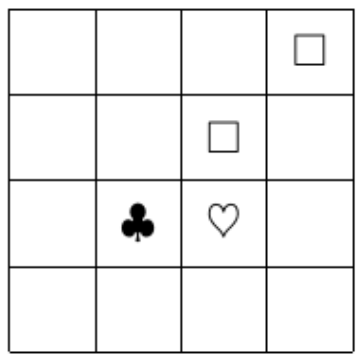
\includegraphics[width=0.2\textwidth]{img/grid_example}
        \caption{Esempio di griglia iniziale}
        \label{fig:grid_ex}
    \end{figure}

    \section{Modello codificato in MiniZinc}\label{sec:modello-codificato-in-minizinc}
    Nel modello MiniZinc i semi e le celle vietate vengono codificati utilizzando degli interi: al seme di cuori corrisponde il numero 1; al seme di fiori corrisponde il numero 2; al seme di picche corrisponde il numero 3; al seme di quadri corrisponde il numero 4; le celle vietate vengono occupate con il numero 5.

    Il modello MiniZinc è costruito in modo da ricevere in input:

    \begin{itemize}
        \item la dimensione della griglia;
        \item il numero di carte disponibile per ogni seme;
        \item il numero di celle bloccate;
        \item una matrice 2D di variabili che rappresenta la griglia iniziale, popolata dalle carte iniziali e dai blocchi.
    \end{itemize}

    \begin{Verbatim}[numbers=left,firstnumber=3,frame=lines,framesep=3mm,label={verb:input}]
    int: n;
    int: hearts;
    int: clubs;
    int: spades;
    int: diamonds;
    int: blocked;
    array[1..n, 1..n] of var 1..5: m;
    \end{Verbatim}

    Una variabile viene utilizzata per salvare il valore del punteggio ad ogni passaggio del processo di ottimizzazione:

    \begin{Verbatim}[numbers=left,firstnumber=10,frame=lines,framesep=3mm,label={verb:score}]
    var int: p;
    \end{Verbatim}

    Per imporre il vincolo di cardinalità su ogni seme (numero di carte disponibile per ogni seme, dato in input) viene utilizzato il vincolo \textit{global\_constraint\_low\_up} con minimo 0 e massimo il valore della variabile corrispondente al seme d'interesse:

    \begin{Verbatim}[numbers=left,firstnumber=12,frame=lines,framesep=3mm,label={verb:cardinality} ,breaklines=true]
    constraint global_cardinality_low_up([m[i,j] | i,j in 1..n], 1..1, [0 | k in 1..1], [hearts | k in 1..1]);
    constraint global_cardinality_low_up([m[i,j] | i,j in 1..n], 2..2, [0 | k in 2..2], [clubs | k in 2..2]);
    constraint global_cardinality_low_up([m[i,j] | i,j in 1..n], 3..3, [0 | k in 3..3], [spades | k in 3..3]);
    constraint global_cardinality_low_up([m[i,j] | i,j in 1..n], 4..4, [0 | k in 4..4], [diamonds | k in 4..4]);
    \end{Verbatim}

    Un vincolo analogo viene utilizzato per impedire a MiniZinc di riempire le celle con il valore 5 (cella vietata):

    \begin{Verbatim}[numbers=left,firstnumber=12,frame=lines,framesep=3mm,label={verb:blocked\_cardinality},breaklines=true]
    constraint global_cardinality_low_up([m[i,j] | i,j in 1..n], 5..5, [0 | k in 5..5], [blocked | k in 5..5]);
    \end{Verbatim}


    Per imporre il vincolo relativo al numero massimo di carte adiacenti dello stesso seme (tre) viene utilizzato un vincolo \textit{forall} unito al costrutto if-then.
    In particolare, si impone che per ogni riga (e colonna), data una cella e due celle consecutive che contengono lo stesso valore della prima, la quarta cella consecutiva alla prima deve contenere un valore diverso (questo non vale per le celle vuote e quelle bloccate):

    \begin{Verbatim}[numbers=left,firstnumber=17,frame=lines,framesep=3mm,label={verb:four\_different},breaklines=true]
    constraint forall(i in 1..n, j in 1..n-3)(
      if m[i,j] == m[i,j+1] /\ m[i,j] == m[i,j+2] /\ m[i,j] != 5
      then m[i,j] != m[i,j+3]
      endif
     );

    constraint forall(j in 1..n, i in 1..n-3)(
      if m[i,j] == m[i+1,j] /\ m[i,j] == m[i+2,j] /\ m[i,j] != 5
      then m[i,j] != m[i+3,j]
      endif
    );
    \end{Verbatim}

    Per il calcolo del punteggio è stato creato un vincolo sulla variabile scelta per racchiudere il punteggio: per ogni possibile combinazione di semi viene verificata un'espressione booleana associata alla combinazione stessa e per ogni occorrenza viene sommato il valore associato (ad esempio sei per il poker orizzontale).
    Di seguito si fornisce un esempio di calcolo del punteggio per la quaterna orizzontale:

    \begin{Verbatim}[numbers=left,firstnumber=30,frame=lines,framesep=3mm,label={verb:horiz\_four},breaklines=true]
    sum(i in 1..n)(
        sum(j in 1..n-3)(
          if
            m[i,j] != 5 /\
            m[i,j+1] != 5 /\
            m[i,j+2] != 5 /\
            m[i,j+3] != 5 /\
            m[i,j] != m[i,j+1] /\
            m[i,j] != m[i,j+2] /\
            m[i,j] != m[i,j+3] /\
            m[i,j+1] != m[i,j+2] /\
            m[i,j+1] != m[i,j+3] /\
            m[i,j+2] != m[i,j+3]
          then 6
          else 0
          endif
        )
    )
    \end{Verbatim}

    Si rimanda al codice sorgente per avere una visione del modello completo e del calcolo del punteggio.

    \section{Modello codificato in ASP}\label{sec:modello-codificato-in-asp}
    Nel modello ASP si è adottata la stessa codifica per i semi e le celle bloccate presentata per il modello codificato in MiniZinc.

    Per il modello ASP sono stati creati i predicati:

    \begin{itemize}
        \item \textit{lato} di arità 1 con range [1,n];
        \item \textit{simbolo} di arità 1 con range [1,5];
        \item \textit{griglia} di arità 3 che rappresenta l'assegnazione alla cella di coordinate (x,y) del simbolo s.
    \end{itemize}

    Per definire le assegnazioni del predicato \textit{griglia} è stato definito il seguente vincolo di cardinalità:

    \begin{Verbatim}[numbers=left,firstnumber=4,frame=lines,framesep=3mm,label={verb:asp\_allocation},breaklines=true]
    {griglia(X,Y,S) : simbolo(S), S != 5} 1:- lato(X), lato(Y), not griglia(X, Y, 5).
    \end{Verbatim}

    Questo garantisce che a ogni step di ottimizzazione venga fatta un'assegnazione (con \textit{S} diverso da 5) per ogni cella che non è bloccata od occupata in partenza (per queste celle viene fornito un apposita assegnazione del predicato \textit{griglia} prima della valutazione del modello).

    Per imporre il vincolo di cardinalità sul numero di carte per ogni seme vengono utilizzati i seguenti vincoli:

    \begin{Verbatim}[numbers=left,firstnumber=4,frame=lines,framesep=3mm,label={verb:asp\_cardinality},breaklines=true]
    :- hearts < #count{X,Y : lato(X), lato(Y), griglia(X,Y,1)}.
    :- clubs < #count{X,Y : lato(X), lato(Y), griglia(X,Y,2)}.
    :- spades < #count{X,Y : lato(X), lato(Y), griglia(X,Y,3)}.
    :- diamonds < #count{X,Y : lato(X), lato(Y), griglia(X,Y,4)}.
    \end{Verbatim}

    Mentre per imporre il vincolo sul numero massimo di carte adiacenti dello stesso seme (tre) vengono utilizzati i seguenti vincoli, rispettivamente per le colonne e per le righe:
    \begin{Verbatim}[numbers=left,firstnumber=4,frame=lines,framesep=3mm,label={verb:asp\_four\_different},breaklines=true]
    :- simbolo(S), lato(X), lato(Y1), lato(Y2), lato(Y3), lato(Y4),
       Y1+1 == Y2, Y1+2 == Y3, Y1+3 == Y4,
       S != 5,
       griglia(X,Y1,S), griglia(X,Y2,S), griglia(X,Y3,S), griglia(X,Y4,S).

    :- simbolo(S), lato(Y), lato(X1), lato(X2), lato(X3), lato(X4),
       X1+1 == X2, X1+2 == X3, X1+3 == X4,
       S != 5,
       griglia(X1,Y,S), griglia(X2,Y,S), griglia(X3,Y,S), griglia(X4,Y,S).
    \end{Verbatim}

    Per il calcolo del punteggio è stato creato il predicato \textit{score} di arità 1 con variabile \textit{P} che rappresenta il punteggio totale.
    Si rimanda al codice sorgente per avere una visione del modello completo e del calcolo del punteggio.

    \section{Test}\label{sec:test}
    Per supportare la fase di test sono stati creati due programmi in C per la generazione d'istanze casuali del problema nei due formati d'input e per raccogliere i risultati dell'esecuzione dei modelli sulle due istanze.

    È stata apportata anche una modifica all'output del modello MiniZinc in modo che coincidesse con quello del modello ASP e il programma C potesse interpretare i risultati in modo uniforme.
    \begin{Verbatim}[numbers=left,firstnumber=4,frame=lines,framesep=3mm,label={verb:output\_mzn},breaklines=true]
    output["griglia(" ++ show(i) ++ "," ++ show(j) ++ "," ++ show(m[i,j]) ++ ") " | i,j in 1..n] ++
    ["\nOptimization: " ++ show(p)]
    \end{Verbatim}

    \subsection{Generazione delle istanze}\label{subsec:generazione-delle-istanze}
    Per la generazione delle istanze casuali è stato creato il programma \textit{setup.c} che prende in input una sequenza di interi corrispondenti alle dimensioni delle griglie da generare e per ogni dimensione genera 20 istanze casuali del problema andando a generare casualmente le celle bloccate e le carte iniziali.
    Per ogni seme viene generato, in modo indipendente, un intero casuale che al più può essere pari al numero di celle totali della griglia.
    Le celle bloccate o occupate possono essere al più un terzo del totale delle celle della griglia.

    Il programma genera un file per ogni istanza sia nel formato MiniZinc che nel formato ASP e li salva nelle sottocartelle dedicate per ogni formato.

    \subsection{Esecuzione dei test}\label{subsec:esecuzione-dei-test}
    Per l'esecuzione dei test è stato creato il programma \textit{benchmark.c} che prende in input una sequenza di interi corrispondenti alle dimensioni delle griglie da testare e per ogni dimensione esegue i modelli MiniZinc e ASP su tutte le istanze generate per quella dimensione.

    L'output generato dai due modelli viene salvato in un file .json appositamente creato per ogni esecuzione dello script.

    \subsection{Parametri di esecuzione}\label{subsec:parametri-di-esecuzione}
    Per l'esecuzione dei test con il modello ASP è stato utilizzato il solver \textit{clingo} con i seguenti parametri: \textit{--time-limit 300 --configuration=jumpy --restart-on-model -t 8,split}.

    Per l'esecuzione dei test con il modello MiniZinc è stato utilizzato il solver \textit{Chuffed} con timeout a 300 secondi, esecuzione parallela su 8 core e mostrando le soluzioni intermedie.
    Tutti i parametri sono disponibili nel file \textit{minizinc/config.mpc}.

    I parametri sono stati scelti dopo una fase di test preliminare in cui sono state analizzate le performance con diversi parametri in particolare variando il parametro \textit{configuration} in ASP e il solver utilizzato da MiniZinc.
    Nella relazione sono presentati i risultati delle configurazioni migliori per questioni di spazio.

    \section{Risultati}\label{sec:risultati}
L'esecuzione dei test è stata effettuata su griglie quadrate di dimensione: 3, 4, 5, 6, 8, 10.
La dimensione massima della griglia è stata posta a 10 in quanto sia la codifica in MiniZinc che quella in ASP hanno mostrato il raggiungimento della soglia dei 300 secondi di esecuzione in tutte e 20 le griglie generate.

\begin{figure}
    \centering
    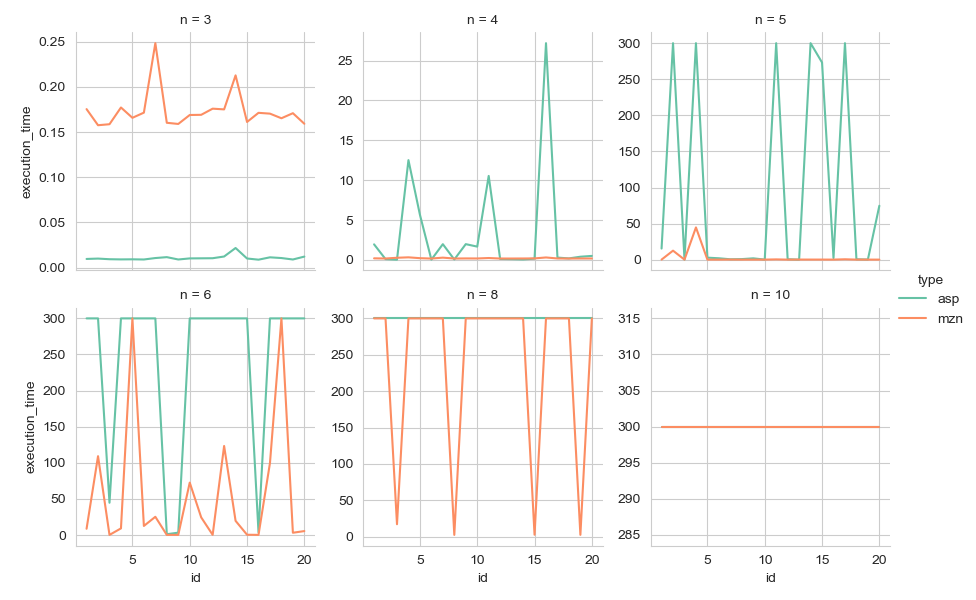
\includegraphics[width=0.8\textwidth]{img/cmpplot}
    \caption{Confronto tra ASP e MiniZinc}
    \label{fig:cmpplot}
\end{figure}

Come visibile dalla figura~\ref{fig:cmpplot}, la codifica in MiniZinc si è rilevata essere più performante rispetto a quella in ASP per le griglie di dimensione superiore a 3, con alcune eccezioni per le griglie di dimensione 4.

La codifica in ASP ha iniziato a saturare il tempo di esecuzione a partire dalla griglia di dimensione 5, mentre la codifica in MiniZinc ha iniziato a saturare il tempo di esecuzione a partire dalla griglia di dimensione 6.

\begin{figure}
    \centering
    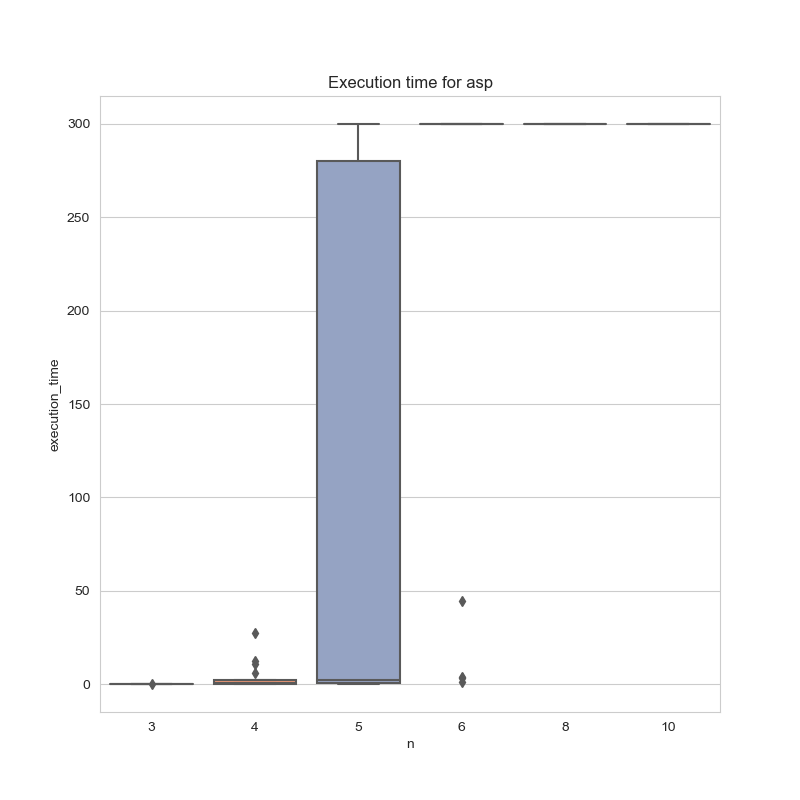
\includegraphics[width=0.5\textwidth]{img/boxplot_asp}
    \caption{Boxplot dei tempi di esecuzione in ASP}
    \label{fig:boxplot_asp}
\end{figure}

\begin{figure}
    \centering
    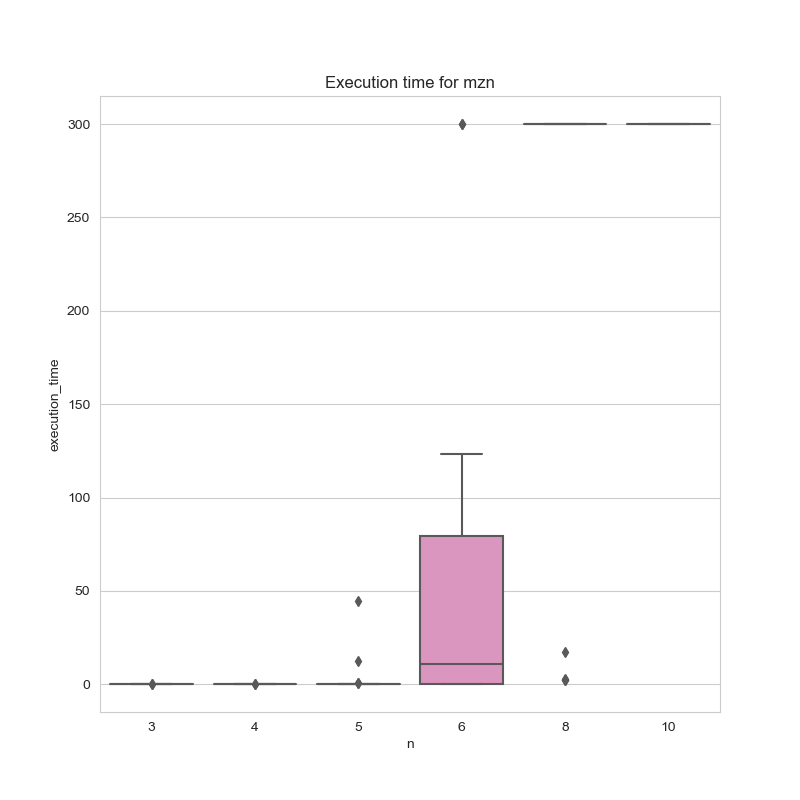
\includegraphics[width=0.5\textwidth]{img/boxplot_mzn}
    \caption{Boxplot dei tempi di esecuzione in MiniZinc}
    \label{fig:boxplot_mzn}
\end{figure}

I boxplot delle figure~\ref{fig:boxplot_asp} e~\ref{fig:boxplot_mzn} mostrano come la codifica in ASP sia meno stabile rispetto a quella in MiniZinc, in quanto i tempi di esecuzione sono molto meno concentrati attorno alla mediana (vedi griglia di dimensione 5 in ASP e griglia di dimensione 6 in MiniZinc).

È stato generato anche un grafico di correlazione per indagare la dipendenza tra il tempo di esecuzione e la dimensione della griglia, il numero di caselle occupate e il numero di caselle libere.

\begin{figure}
    \centering
    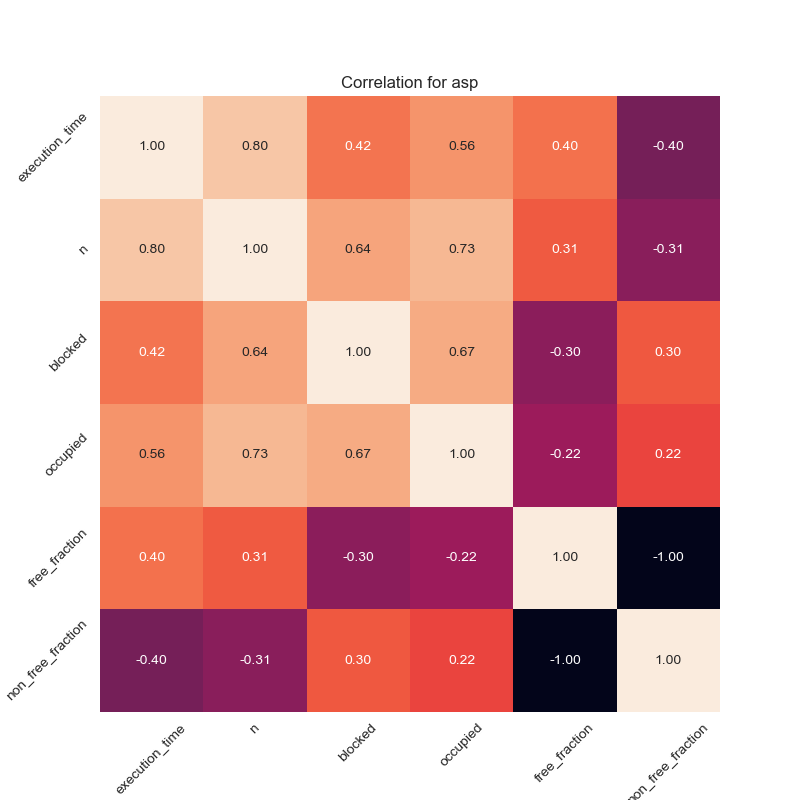
\includegraphics[width=0.5\textwidth]{img/correlation_asp}
    \caption{Grafico di correlazione per ASP}
    \label{fig:correlation_asp}
\end{figure}

\begin{figure}
    \centering
    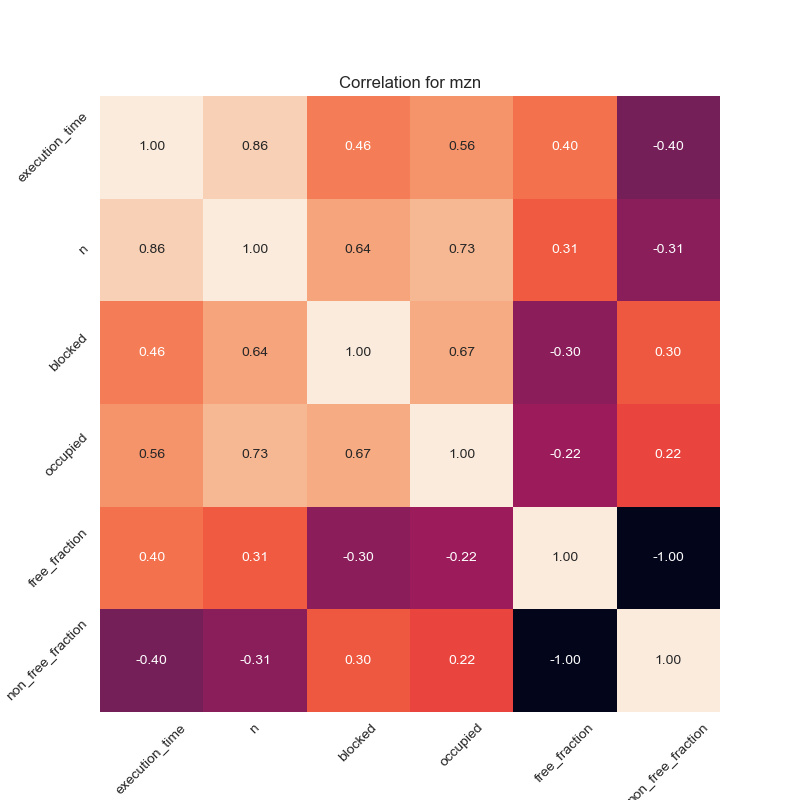
\includegraphics[width=0.5\textwidth]{img/correlation_mzn}
    \caption{Grafico di correlazione per MiniZinc}
    \label{fig:correlation_mzn}
\end{figure}

Come riportato in entrambi i grafici di correlazione (figure~\ref{fig:correlation_asp} e~\ref{fig:correlation_mzn}), il tempo di esecuzione è fortemente correlato con la dimensione della griglia, mentre c'è un moderato livello di correlazione con il numero di caselle occupate e il numero di caselle libere.
Questo può essere dovuto al fatto che aumentando la dimensione della griglia aumenta notevolmente il livello di difficoltà del problema mentre il numero di caselle occupate rimane una frazione (massimo 1/3) del numero di caselle totali.

A scopo di completezza, è stata creata una breve animazione che mostra una comparativa della risoluzione della griglia numero 15 di dimensione 5 nelle due codifiche proposte.
L'animazione è disponibile su YouTube al seguente \href{https://youtu.be/e243VU-qNLE}{indirizzo}.

\end{document}